\model{List Interface}
% Based on Model 1 of Lists activity by Clif Kussmaul

In computer science, a \textit{list} is a sequence of items with an \textit{index} (or position) for each item.

\begin{center}
\begin{tabular}{|c|c|c|c|c|c|c|c|c|c|}
\hline
\tr \textbf{index:} & 0 & 1 & 2 & 3 & 4 & 5 & 6 & 7 & \ldots \\
\hline
\tr \textbf{item:} & \str{Mer} & \str{Ven} & \str{Ear} & \str{Mar} & \str{Jup} & \str{Sat} & \str{Ura} & \str{Nep} & \ldots \\
\hline
\end{tabular}
\end{center}

Since we know which item is first, second, etc., we say that the list is \textit{ordered}.
%This does \textbf{not} mean that the items have been sorted in any way.
The first item is at the \textit{head} of the list; the last item is at the \textit{tail} of the list.
Here is a subset of methods from \java{interface List<E>} in the Java API.

\begin{center}
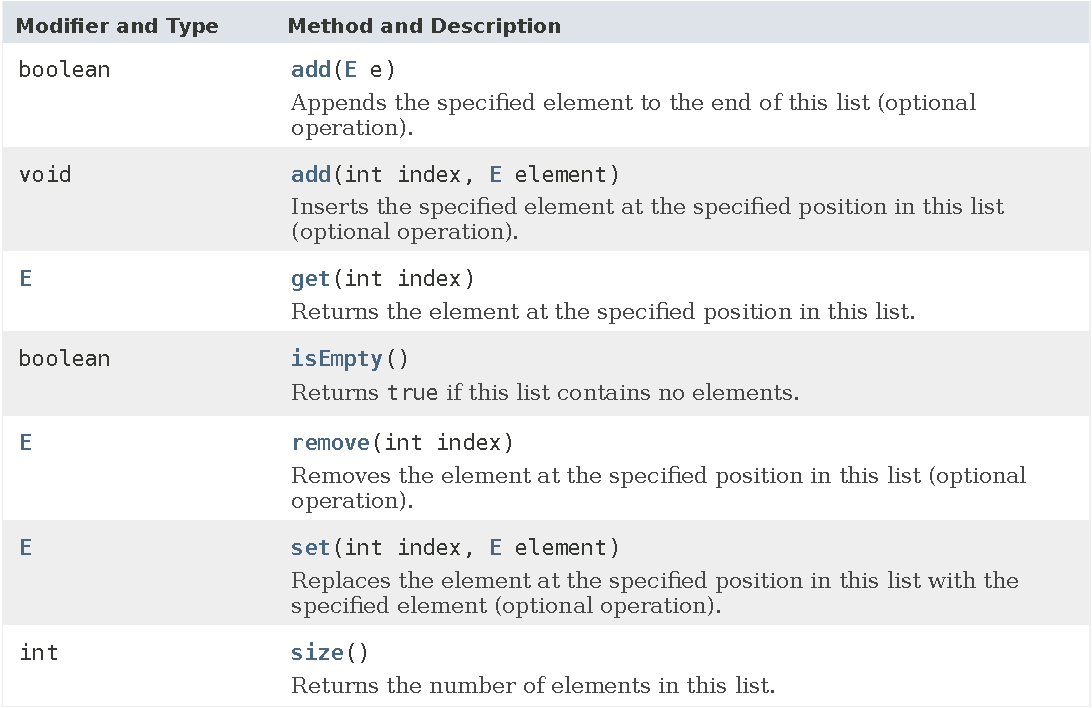
\includegraphics[width=0.85\linewidth]{figs/ListAPI.pdf}
\end{center}


\quest{10 min}


\Q Give several examples of lists from everyday life.

\begin{answer}
Grocery list, playlist on Spotify, to-do lists, etc.
\end{answer}


\Q What is the index of the head of a list?
In general, what is the index of the tail of a list?

\begin{answer}[3em]
The head is at index 0, the tail is at index size - 1.
\end{answer}


\Q In Java lists, what does the \java{<E>} represent?

\begin{answer}
\java{<E>} is a generic type, i.e., the type of the list items.
Notice that \java{add} takes an \java{E} as a parameter, and \java{get} returns an element of type \java{E}.
\end{answer}


\Q Of the seven methods shown from the Java API, how many change the contents of the list?

\begin{answer}[3em]
Four: \java{add} (at the end), \java{add} (at a position), \java{remove}, and \java{set}.
\end{answer}


\Q \label{listtable}
Fill in the table below to show the contents of the list after each method call.
Note that the \java{add} method returns \java{true} if the list changes as a result, and the \java{set} method returns the element previously at the specified position.

\begin{center}
\begin{tabular}{|l|C{4pt}|C{24pt}|C{24pt}|C{24pt}|C{24pt}|C{24pt}|C{4pt}|c|}
\hline
\tr Method Call      & \tg & \tr  0  & \tr  1  & \tr  1  & \tr  3  & \tr 4 & \tg & \tr Return Value \\
\hline
\java{add(0, "A")}   & \tg &      A  &         &         &         &       & \tg & true \\
\hline
\java{size()}        & \tg &      A  &         &         &         &       & \tg & 1 \\
\hline
\java{add("N")}      & \tg &      A  &      N  &         &         &       & \tg & true \\
\hline
\java{add(0, "R")}   & \tg & \ans{R} & \ans{A} & \ans{N} &         &       & \tg & \ans{true} \\
\hline
\java{add("G")}      & \tg & \ans{R} & \ans{A} & \ans{N} & \ans{G} &       & \tg & \ans{true} \\
\hline
\java{size()}        & \tg & \ans{R} & \ans{A} & \ans{N} & \ans{G} &       & \tg & \ans{4} \\
\hline
\java{remove(0)}     & \tg & \ans{A} & \ans{N} & \ans{G} &         &       & \tg & \ans{R} \\
\hline
\java{get(0)}        & \tg & \ans{A} & \ans{N} & \ans{G} &         &       & \tg & \ans{A} \\
\hline
\java{get(size()-1)} & \tg & \ans{A} & \ans{N} & \ans{G} &         &       & \tg & \ans{G} \\
\hline
\java{set(1, "U")}   & \tg & \ans{A} & \ans{U} & \ans{G} &         &       & \tg & \ans{N} \\
\hline
\end{tabular}
\end{center}


\Q When adding or removing elements at the beginning, what did you have to do with the existing elements in the list?

\begin{answer}
To keep the list in order, existing elements need to be shifted down by one to the right for adding and to the left for removing.
\end{answer}


\Q In your own words, describe what a \java{List} collection is from a programmer's perspective.

\begin{answer}[5em]
A \java{List} is an ordered collection of elements (also known as a sequence).
The user of this interface has precise control over where  each element is inserted.
You can access elements by their integer index and search for elements in the list.
\end{answer}
